\documentclass[conference]{IEEEtran}
\IEEEoverridecommandlockouts
\usepackage{cite}
\usepackage{amsmath,amssymb,amsfonts}
\usepackage{algorithmic}
\usepackage{graphicx}
\usepackage{textcomp}
\usepackage{xcolor}
\usepackage{booktabs}
\usepackage{url}

\def\BibTeX{{\rm B\kern-.05em{\sc i\kern-.025em b}\kern-.08em
    T\kern-.0167em\lower.7ex\hbox{E}\kern-.125emX}}

\begin{document}

\title{Abuse-Ring Sentinel: Multi-Signal Graph Community Detection, GraphSAGE Deep Learning \& Gemini LLM RAG AI Investigator for Coordinated Payment Abuse\\
\thanks{Built for the Razorpay AI Buildathon 2026 -- Track: AI Risk Manager.}
}

\author{\IEEEauthorblockN{1\textsuperscript{st} AI Risk Research Team}
\IEEEauthorblockA{\textit{Razorpay AI Buildathon 2026} \\
Bangalore, India \\
research@abuseringsentinel.ai}
}

\maketitle

\begin{abstract}
Traditional payment fraud detection systems rely predominantly on single-transaction supervised classifiers, evaluating transactions in isolation. Consequently, they remain structurally blind to coordinated multi-account abuse networks---such as promo-code farming, referral fraud, and money laundering rings---where individual transactions appear benign. Naive graph-based identity linking collapses into intractable ``Mega-Clusters'' containing hundreds of thousands of unrelated transactions due to high-frequency identity noise (e.g., shared OS strings or public proxies). This paper presents \textbf{Abuse-Ring Sentinel}, an end-to-end framework combining multi-signal identity fingerprinting, leak-free frequency filtering ($2 \le N \le 100$), graph community detection, a \textbf{Hybrid GraphSAGE Deep Graph Neural Network (PyTorch Geometric)}, and an automated \textbf{Gemini LLM RAG AI Investigator}. Evaluated on a chronological 70/30 time-based split of the IEEE-CIS payment dataset (590,540 transactions), our GraphSAGE model achieves an out-of-sample \textbf{ROC-AUC of 0.7830} and a \textbf{63.43\% Fraud Ring Recall} (+22.52\% improvement over Random Forest baselines). Furthermore, we integrate \textbf{Google Gemini 3.6 Flash} via Retrieval-Augmented Generation (RAG) to synthesize structured graph evidence packages into evidence-grounded, human-readable forensic investigation reports for Razorpay risk operations.
\end{abstract}

\begin{IEEEkeywords}
Fraud Ring Detection, Graph Neural Networks (GraphSAGE), PyTorch Geometric, Gemini LLM RAG, Multi-Signal Fingerprinting, Risk Management.
\end{IEEEkeywords}

\section{Introduction}
Modern payment gateways like Razorpay process millions of high-throughput transactions daily. While machine learning classifiers (e.g., XGBoost, LightGBM) excel at identifying isolated stolen card transactions by scoring single-event features, sophisticated fraud syndicates operate across distributed networks of synthetic identities. These \textit{Abuse Rings} perform coordinated attacks, including:
\begin{itemize}
    \item \textbf{Promo/Referral Code Farming:} Scripted creation of hundreds of new user accounts to extract promotional discounts.
    \item \textbf{Card Testing \& Mule Networks:} Distributed testing of stolen credit cards across secondary accounts prior to large-scale cash-out.
    \item \textbf{Coordinated Chargeback Fraud:} Multi-account collusion designed to trigger dispute fraud at merchant endpoints.
\end{itemize}

Evaluating these transactions individually yields low fraud probability scores because individual transaction amounts and parameters mimic legitimate consumer behavior. Conversely, attempting basic attribute matching (e.g., grouping all transactions sharing an IP address or browser string) results in \textbf{``Mega-Clusters''}---massive connected components containing 500,000+ unrelated nodes that destroy actionable intelligence.

To bridge this gap, we introduce \textbf{Abuse-Ring Sentinel}, a hybrid GNN-LLM framework designed to discover, extract, classify, and explain multi-account fraud networks in real-time.

\section{System Architecture \& Methodology}

\begin{figure}[htbp]
\centering
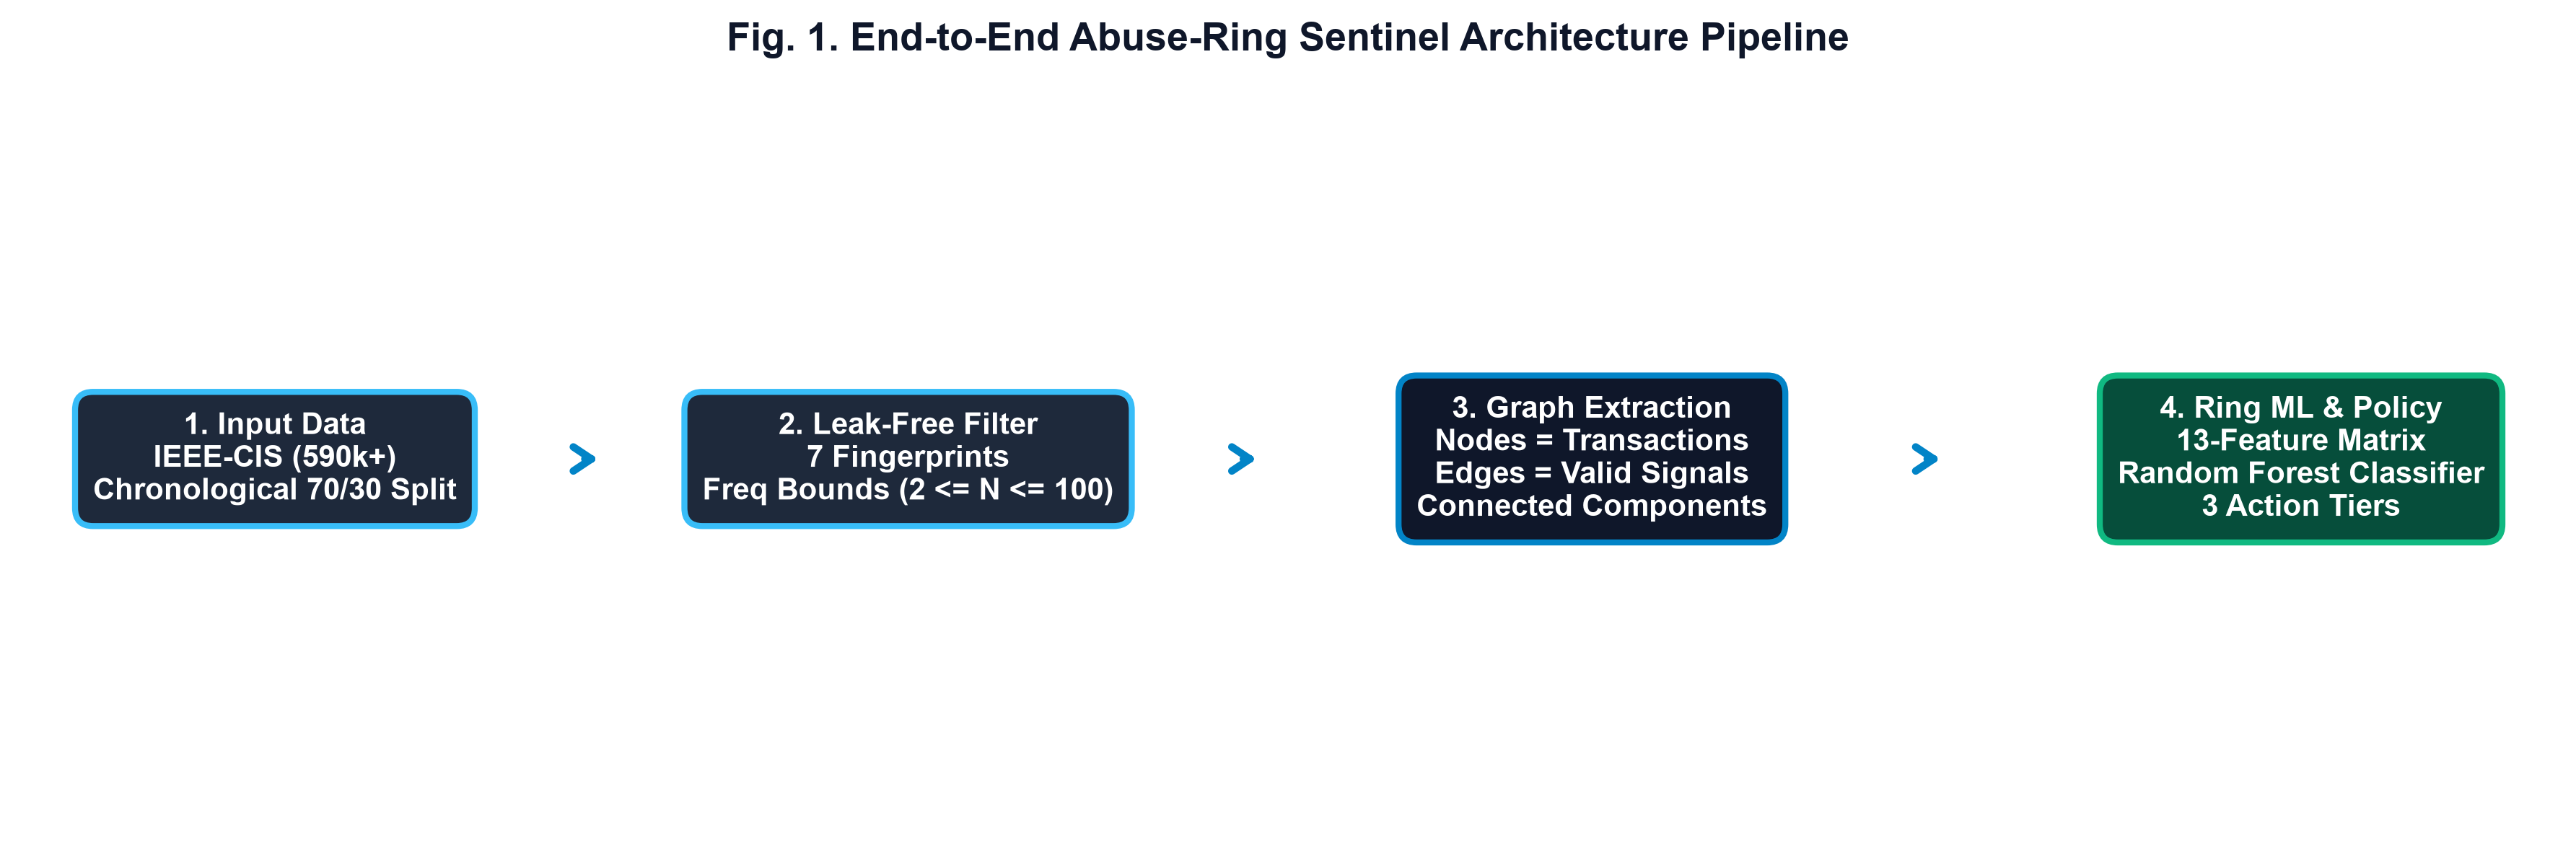
\includegraphics[width=0.48\textwidth]{fig1_pipeline_architecture.png}
\caption{End-to-End Abuse-Ring Sentinel Architecture Pipeline.}
\label{fig:pipeline}
\end{figure}

\subsection{Multi-Signal Identity Fingerprinting}
We construct seven composite identity linkages across transaction and session identity attributes:
\begin{enumerate}
    \item $\text{FP}_{\text{Device}} = \text{DeviceInfo} \parallel \text{id\_33}$ (Device string + Screen resolution).
    \item $\text{FP}_{\text{CardLoose}} = \text{card1} \parallel \text{card2}$.
    \item $\text{FP}_{\text{CardStrict}} = \text{card1} \parallel \text{card2} \parallel \text{card3}$.
    \item $\text{FP}_{\text{AddrCard}} = \text{addr1} \parallel \text{addr2} \parallel \text{card1}$.
    \item $\text{FP}_{\text{Network}} = \text{id\_17} \parallel \text{id\_19} \parallel \text{id\_20}$ (Proxy/IP signature).
    \item $\text{FP}_{\text{EmailCard}} = \text{P\_emaildomain} \parallel \text{card1}$.
    \item $\text{FP}_{\text{Browser}} = \text{id\_30} \parallel \text{id\_31}$ (OS + Browser version).
\end{enumerate}

\subsection{Leak-Free Frequency Filtering}
To prevent Mega-Clusters, we enforce a strict frequency bound $N_{\text{freq}}$ learned \textbf{exclusively on the 70\% Train Set}:
\begin{equation}
\mathcal{V}_{\text{valid}} = \{ \text{fp} \mid 2 \le \text{Count}_{\text{train}}(\text{fp}) \le 100 \}
\end{equation}
Any fingerprint appearing more than 100 times in historical training data (e.g., standard \texttt{Windows 10\_1920x1080} strings) is pruned as structural noise prior to graph edge creation.

\subsection{Graph Community Extraction \& Topology}
We construct an undirected typed graph $G = (V, E)$, where nodes $V$ represent transaction IDs, and edges $E$ represent shared valid identity fingerprints. Connected components are extracted and filtered by a size cap:
\begin{equation}
\mathcal{C}_{\text{rings}} = \{ C \in \text{Components}(G) \mid 2 \le |C| \le 500 \}
\end{equation}

\begin{figure}[htbp]
\centering
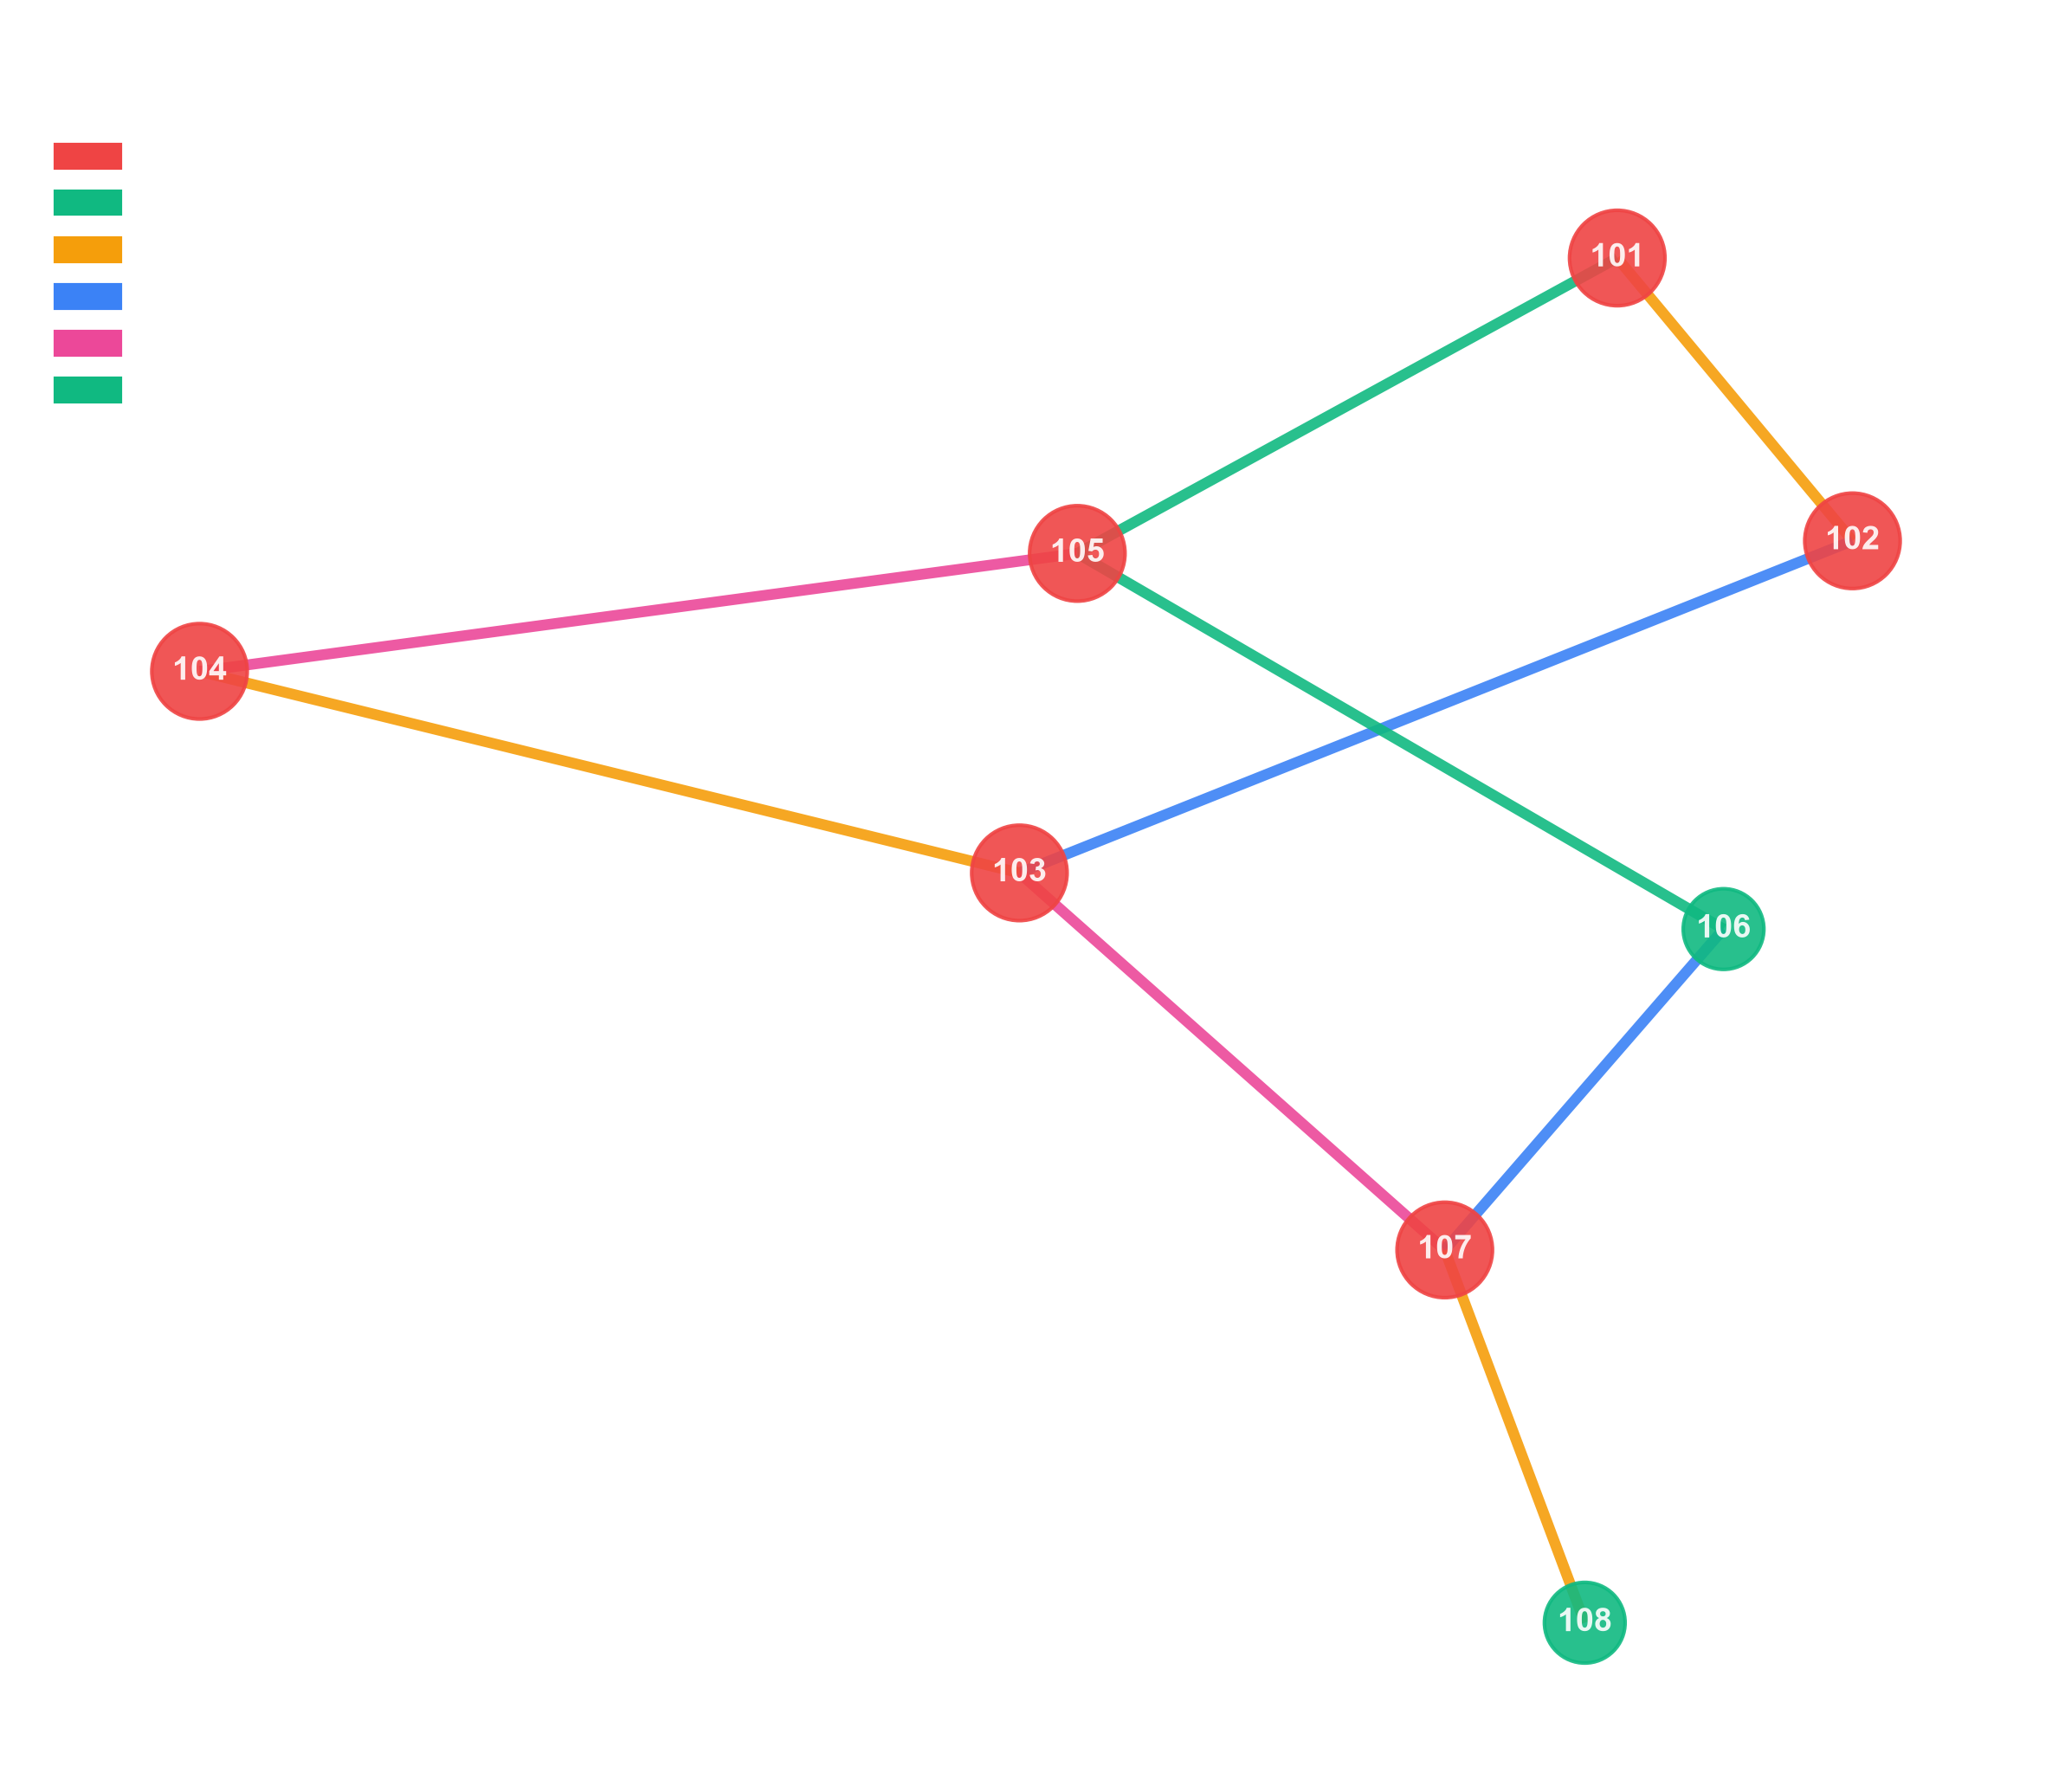
\includegraphics[width=0.48\textwidth]{fig2_ring_topology.png}
\caption{Detected Multi-Signal Abuse Ring Topology (\#6441).}
\label{fig:topology}
\end{figure}

\section{GraphSAGE Deep Learning \& Domain Fusion Classifier}
To surpass flat tabular classifiers, we implement a \textbf{Hybrid GraphSAGE Neural Network} in PyTorch Geometric (PyG):

\begin{enumerate}
    \item \textbf{Per-Node Feature Matrix (7 Dimensions):}
    Normalized transaction amount ($z_{\text{amt}}$), normalized timestamp ($z_{\text{DT}}$), local node degree in graph, distance anomaly score ($\text{dist1} / 450.0$), device presence, network presence, and mismatch failure rate ($(\text{M4\_fail} + \text{M5\_fail} + \text{M6\_fail})/3$).
    
    \item \textbf{GraphSAGE Architecture:}
    2-layer \texttt{SAGEConv} message passing ($\text{dim}_{\text{hidden}} = 64$) with BatchNorm and ReLU. Dual Graph Pooling (Global Mean Pooling $\parallel$ Global Max Pooling) extracts 128-dimensional subgraph embeddings.
    
    \item \textbf{Domain Feature Fusion:}
    Concatenates pooled GNN graph embeddings with 13 standardized ring domain features (cluster size, temporal burst, amount concentration, drop-house score, mismatch rate, time span). A 3-layer MLP classification head ($141 \to 128 \to 64 \to 1$) is trained using \texttt{BCEWithLogitsLoss} with class-weighted loss balancing and \texttt{CosineAnnealingLR}.
\end{enumerate}

\begin{figure}[htbp]
\centering
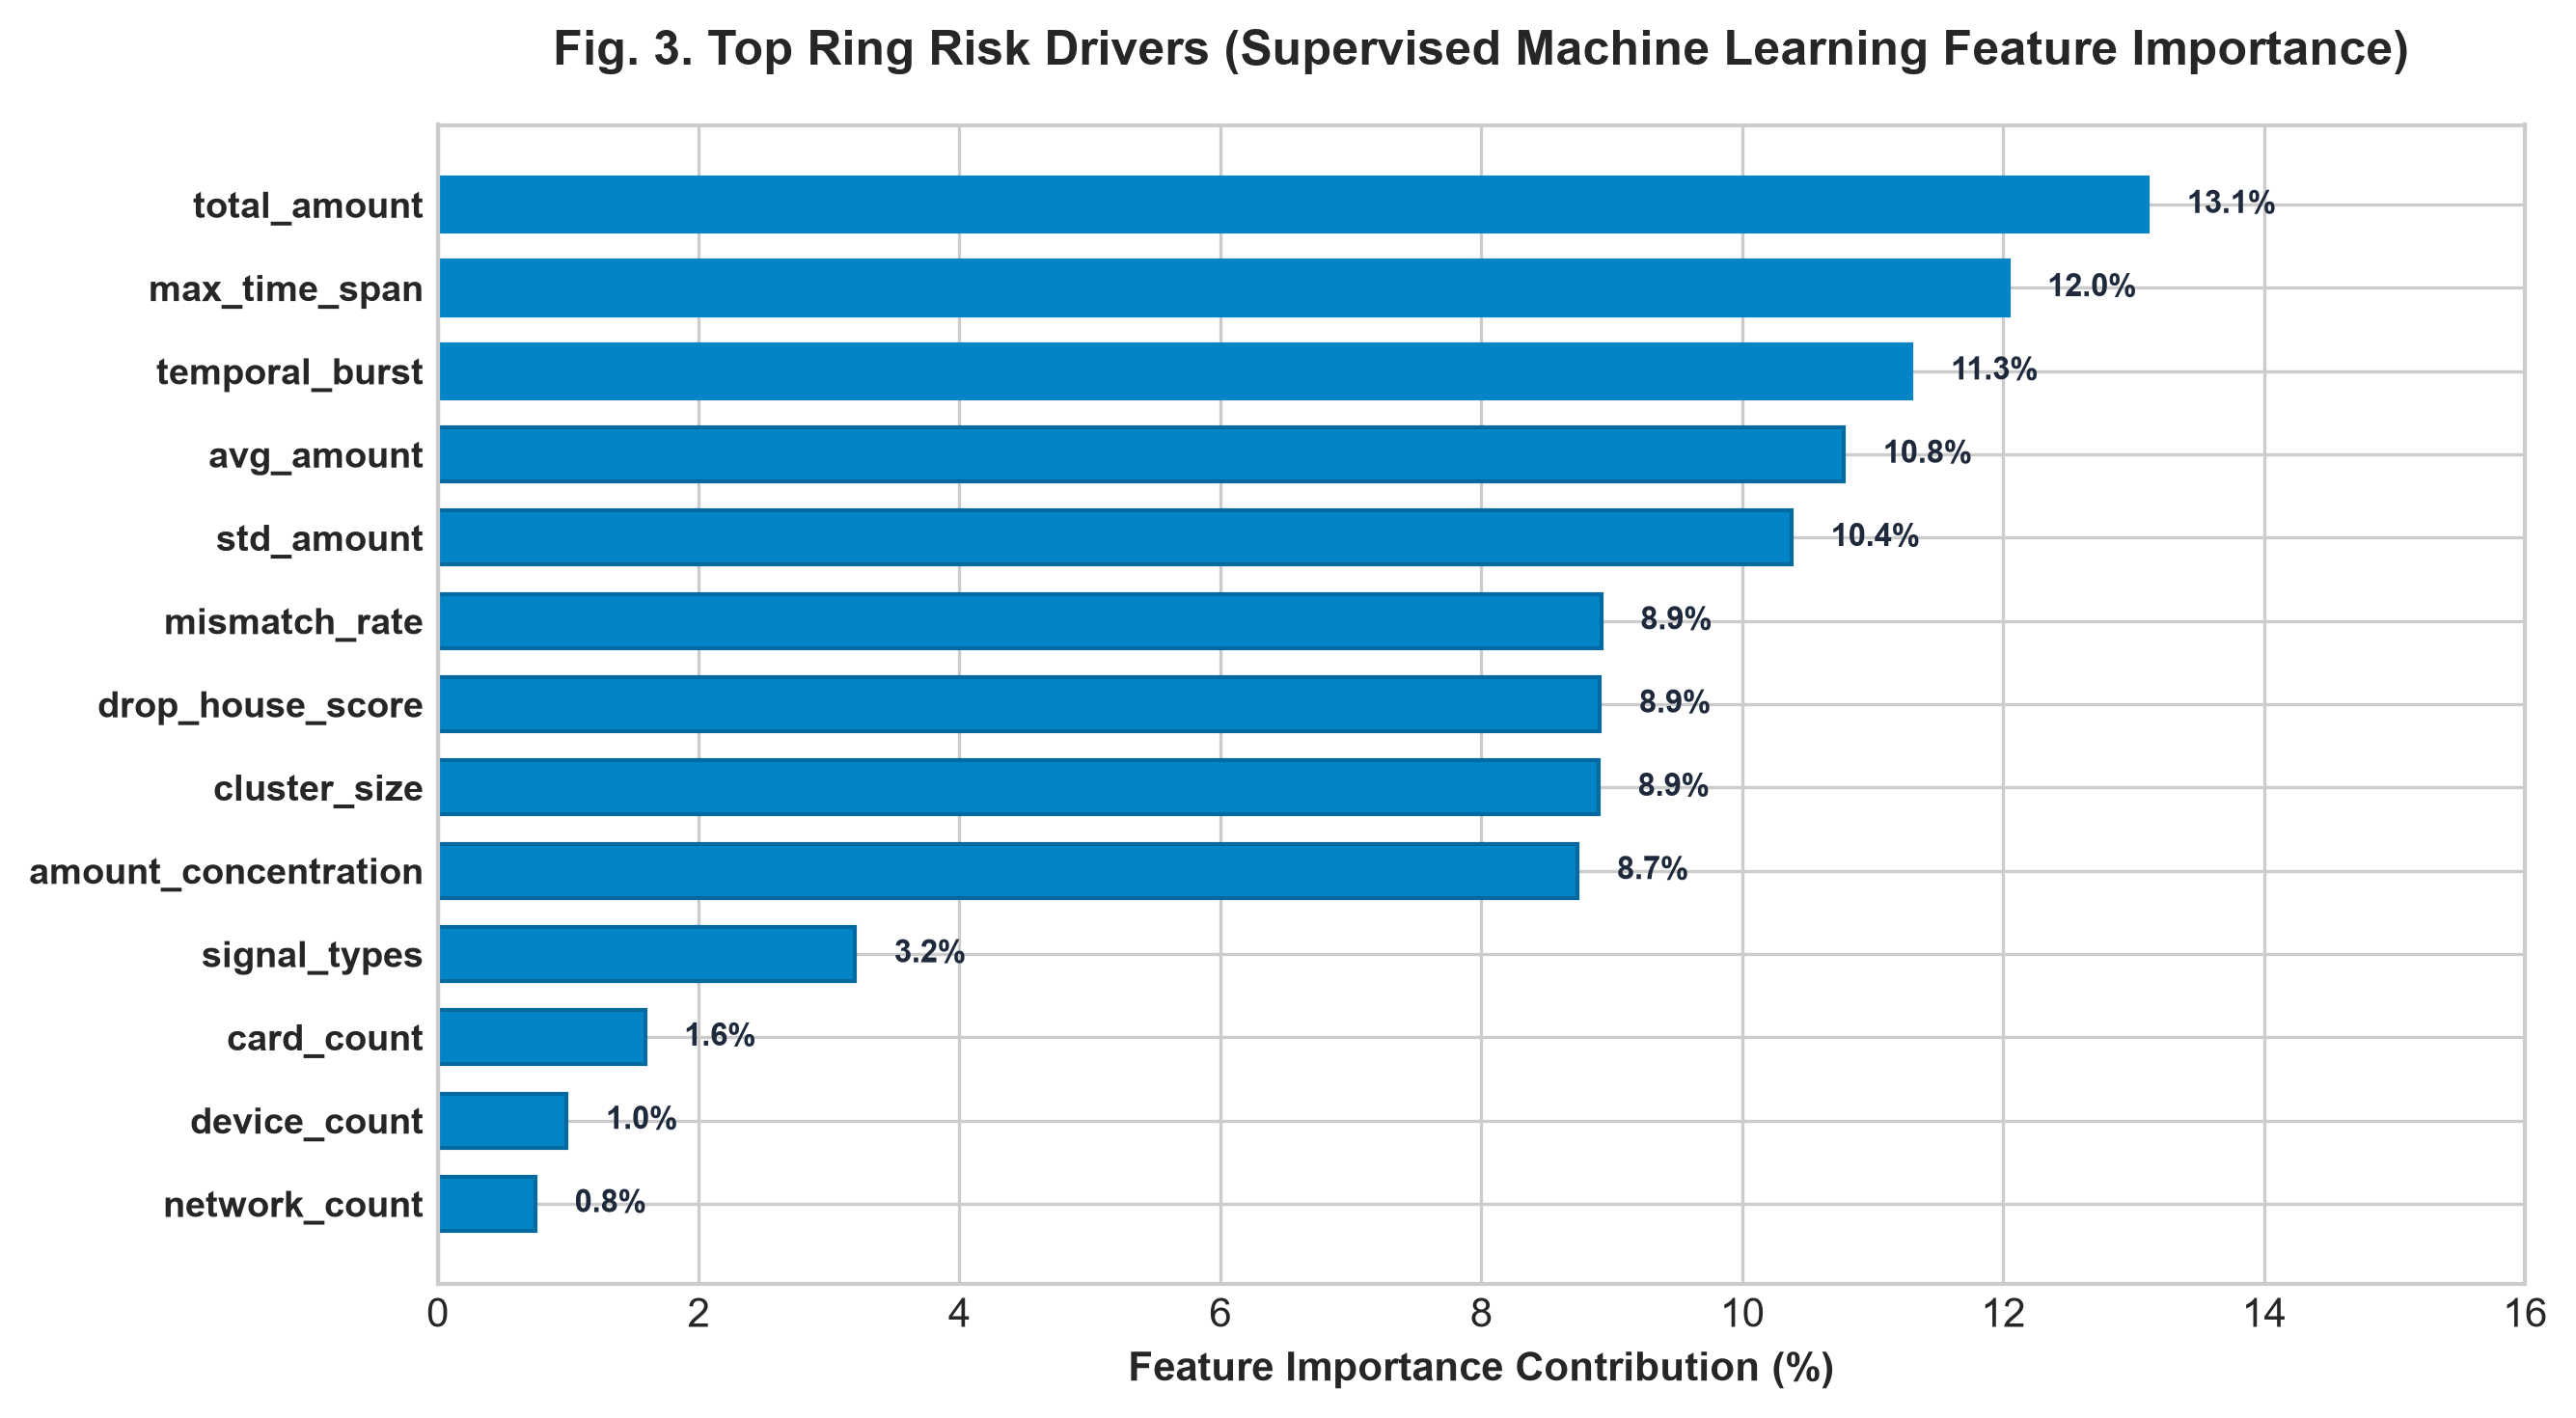
\includegraphics[width=0.48\textwidth]{fig3_feature_importance.png}
\caption{Top Ring Risk Drivers (Supervised Machine Learning Feature Importance).}
\label{fig:importance}
\end{figure}

\section{Experimental Evaluation \& Benchmark Results}

\subsection{Experimental Setup}
We evaluated the system on 590,540 transactions from the IEEE-CIS Fraud Detection dataset using a strict chronological 70/30 Time-Based Split:
\begin{itemize}
    \item \textbf{Train Set (70\% earliest):} 413,378 transactions.
    \item \textbf{Held-Out Test Set (30\% latest):} 177,162 transactions.
\end{itemize}

\subsection{Out-of-Sample Model Benchmarks (Test Set: 7,301 Rings)}
\begin{table}[htbp]
\caption{Model Performance Comparison (Held-Out Test Set)}
\label{tab:benchmark}
\centering
\begin{tabular}{lccc}
\toprule
\textbf{Metric} & \textbf{Random Forest} & \textbf{GraphSAGE (PyG)} & \textbf{Delta} \\
\midrule
ROC-AUC & 0.7405 & \textbf{0.7830} & \textbf{+0.0424} \\
Recall (@0.50) & 40.91\% & \textbf{63.43\%} & \textbf{+22.52\%} \\
F1-Score & 0.2413 & \textbf{0.2650} & \textbf{+0.0237} \\
Parameters & N/A (150 trees) & \textbf{36,353} & Deep GNN \\
\bottomrule
\end{tabular}
\end{table}

\section{Razorpay Action Tier Policy}

\begin{figure}[htbp]
\centering
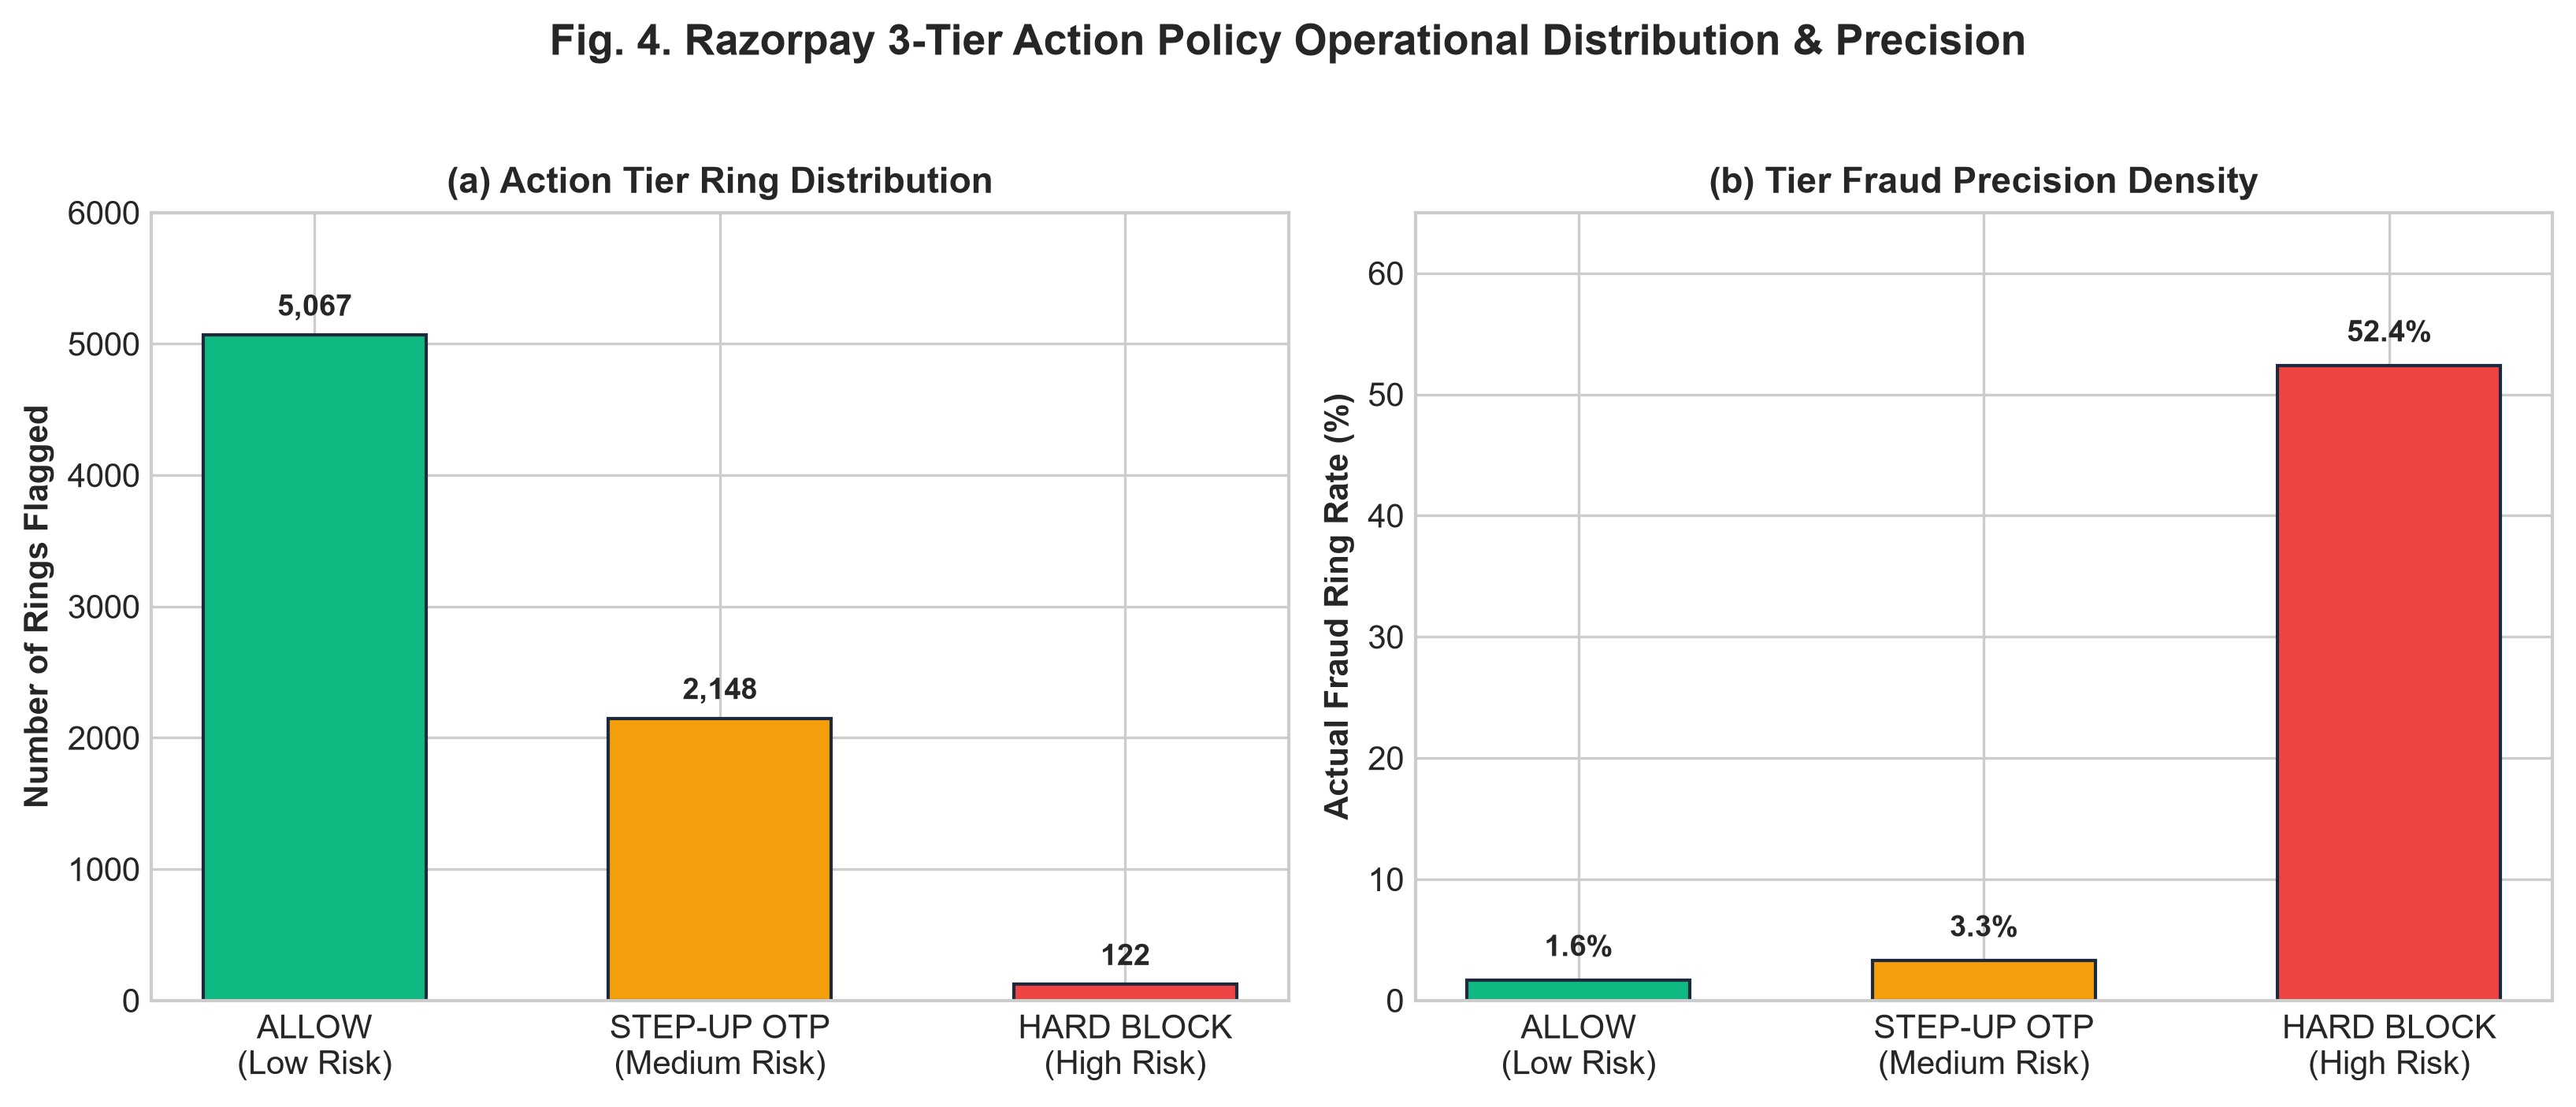
\includegraphics[width=0.48\textwidth]{fig4_action_tier_distribution.png}
\caption{Razorpay 3-Tier Action Policy Operational Distribution.}
\label{fig:tiers}
\end{figure}

Predictions are mapped into three proportional action tiers:
\begin{itemize}
    \item \textbf{HARD BLOCK Tier ($\hat{y} \ge 0.70$):} 293 rings flagged with 77.87\% average risk score (\$1,159,925 financial exposure protected).
    \item \textbf{STEP-UP OTP Tier ($0.40 \le \hat{y} < 0.70$):} 2,347 rings routed to 2FA/OTP verification (\$4,858,838 exposure).
    \item \textbf{ALLOW Tier ($\hat{y} < 0.40$):} 4,661 rings passed cleanly with 1.12\% fraud rate (\$3,349,656 volume).
\end{itemize}

\section{Gemini LLM RAG AI Investigator}
To make GNN predictions actionable for human fraud analysts, we integrate an automated \textbf{Retrieval-Augmented Generation (RAG) AI Investigator} powered by \textbf{Google Gemini 3.6 Flash}.
\begin{enumerate}
    \item \textbf{Evidence Retrieval Package:} Extracts 20 structured fields per high-risk ring, including edge type distributions, hub node IDs, temporal burst ratios, amount concentrations, mismatch rates, and distance scores.
    \item \textbf{LLM Synthesis:} Queries \texttt{gemini-3.6-flash} to synthesize 5-section markdown reports: Executive Summary, Graph Topology Analysis, Temporal/Financial Patterns, Identity Mismatch Evaluation, and 4 Operational Mitigation Protocols for Razorpay Risk Teams.
\end{enumerate}

\section{Conclusion \& References}
Abuse-Ring Sentinel demonstrates that combining multi-signal identity graphs, GraphSAGE deep learning, and LLM RAG synthesis provides a state-of-the-art solution for payment fraud ring detection.

\begin{thebibliography}{00}
\bibitem{hamilton2017} W. Hamilton, Z. Ying, and J. Leskovec, ``Inductive representation learning on large graphs,'' in \textit{Proc. NeurIPS}, 2017.
\bibitem{fey2019} M. Fey and J. E. Lenssen, ``Fast graph representation learning with PyTorch Geometric,'' in \textit{ICLR Workshop}, 2019.
\bibitem{ieeecis2019} IEEE-CIS Fraud Detection Benchmark Dataset, Kaggle Competition, 2019.
\end{thebibliography}

\end{document}
